\section{Functional Modeling}

Functional modeling represents the system-centric view of system analysis, focusing on how data is stored, structured, moved, and transformed within the application. While use case modeling details user-system boundaries and behaviors from the actor's viewpoint, functional modeling defines the logical structures and information pipelines required to make those behaviors possible. In the design of the AI-Driven Lab Exam Monitoring and Management System, functional modeling is particularly important because the system must handle highly dynamic, concurrent data streams (such as real-time process events, webcam frames, and code compilations) while maintaining relational consistency for grades, seating configurations, and immutable security audit logs.

This section provides a rigorous definition of the system's database schema and data flow processes. The Entity Relationship Diagram (ERD) outlines the relational architecture of the system, defining the entities, attributes, primary/foreign keys, and cardinalities that structure the Neon PostgreSQL database. The Data Flow Diagrams (DFDs) at Level 0, Level 1, and Level 2 map the system's operational pathways, demonstrating how telemetry data, user inputs, grading commands, and reporting templates flow between client applications, external services, processing components, and database storage.

\subsection{Entity Relationship Diagram}

The database schema of the SmartExam platform is designed to be highly normalized, adhering to Third Normal Form (3NF) to prevent data redundancy and ensure transactional integrity during high-concurrency examination sessions. Relational integrity is enforced using foreign key constraints, unique indexing, and database-level cascading policies where appropriate. The database layer is hosted on Neon PostgreSQL, providing serverless scalability to handle spikes in database connections when hundreds of workstation clients synchronize telemetry data simultaneously.

The Entity Relationship Diagram (ERD) for the AI-Driven Lab Exam Monitoring and Management System is shown in Figure~\ref{fig:erd_diagram}. It comprises 14 core relational tables that capture the complete operational state of the system:

\begin{figure}[H]
\centering
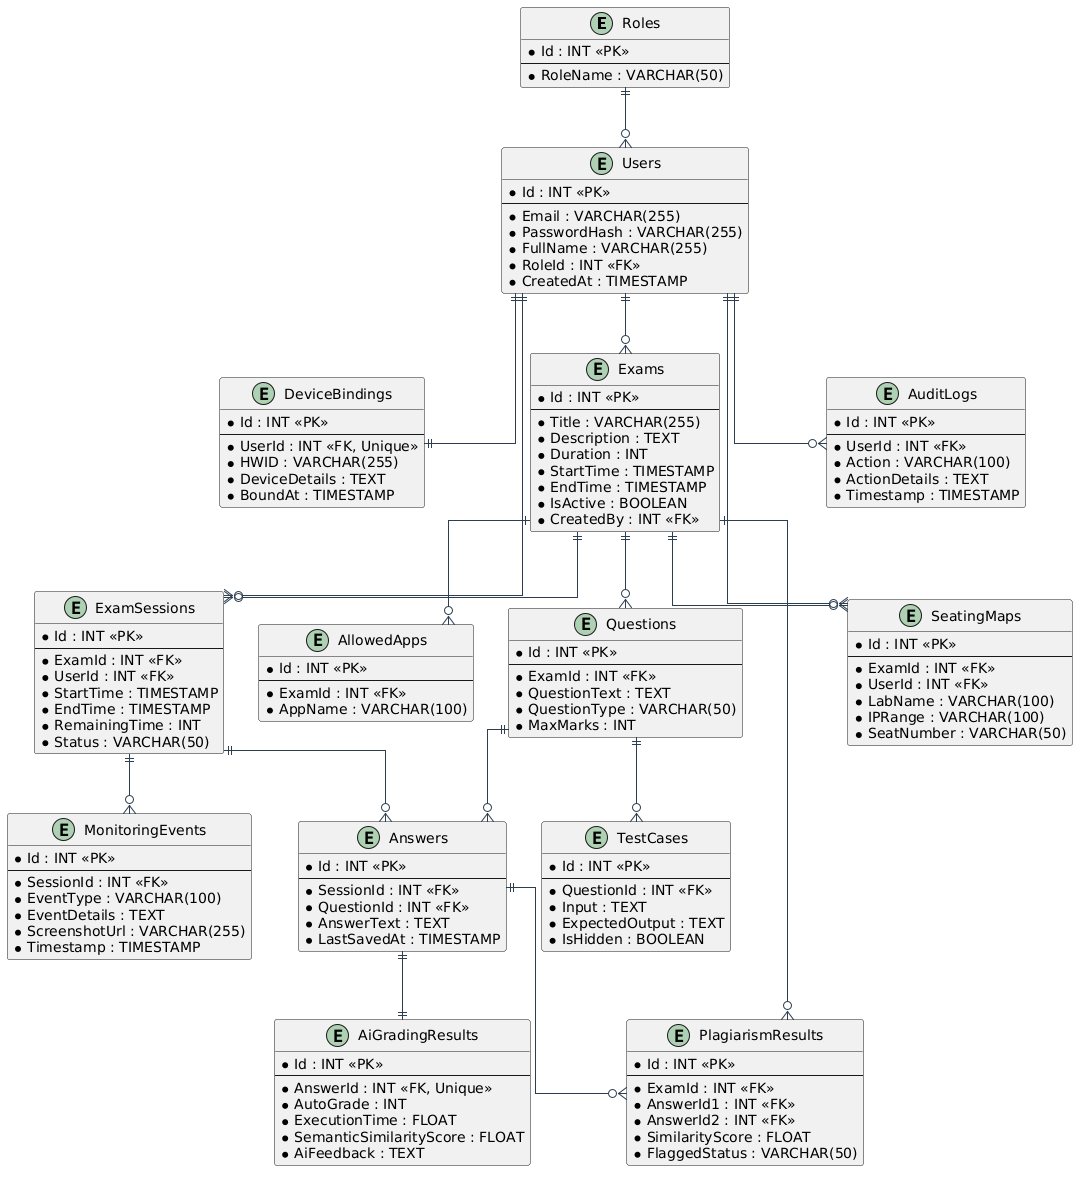
\includegraphics[width=0.97\linewidth]{Figures/erd_diagram.png}
\caption{Entity Relationship Diagram (ERD) of the SmartExam Database Schema}
\label{fig:erd_diagram}
\end{figure}

The relational architecture illustrated in Figure~\ref{fig:erd_diagram} is structured around the following entity groups and relationships:

\begin{enumerate}
    \item \textbf{User and Access Management:} The \texttt{Users} table stores credentials, names, and emails for all participants. It is associated with the \texttt{Roles} table via a many-to-many junction table to enforce Role-Based Access Control (RBAC). The \texttt{DeviceBindings} table forms a one-to-one relationship with the \texttt{Users} table, storing the unique Hardware ID (HWID) string associated with each student. This binding restricts student login to a single registered workstation.
    \item \textbf{Exam and Environment Configuration:} The \texttt{Exams} table is the primary entity for assessment metadata, storing fields such as title, description, duration, start time, end time, and status. It is associated with the \texttt{AllowedApps} table in a one-to-many relationship, defining the whitelist of executable names allowed during lockdown. The \texttt{Questions} table maintains a one-to-many relationship with the \texttt{Exams} table, storing individual exam tasks. For programming questions, the \texttt{TestCases} table links to \texttt{Questions} in a one-to-many relationship, storing the inputs, expected outputs, and visibility flags (public vs. hidden) for auto-compilation.
    \item \textbf{Access Control and Seating Mapping:} The \texttt{SeatingMaps} table manages physical lab allocations. It links to both \texttt{Exams} and \texttt{Users} (Students) to map each candidate to a specific laboratory name, workstation IP address, and seat number, ensuring physical access control.
    \item \textbf{Exam Sessions and Live Telemetry:} When a student launches an exam, a record is created in the \texttt{ExamSessions} table (one-to-many with \texttt{Exams} and \texttt{Users}), tracking start/end times and current progress state. The \texttt{Answers} table links to \texttt{ExamSessions} and \texttt{Questions} to store student inputs, which are auto-saved incrementally. The \texttt{MonitoringEvents} table maps to \texttt{ExamSessions} in a one-to-many relationship, capturing live proctoring telemetry including screenshots (stored as secure S3 blob URLs), running processes list, focus loss events, and camera alert histories.
    \item \textbf{Evaluation and Audit Trails:} The \texttt{AiGradingResults} table links to \texttt{Answers} to store the auto-compilation pass rates, execution speeds, and semantic similarity evaluations. The \texttt{PlagiarismResults} table stores pairwise similarity scores flagged during cross-submission text/code comparisons. Finally, the \texttt{AuditLogs} table acts as an immutable ledger, recording all administrative updates, override commands, and credentials modifications to guarantee system auditability.
\end{enumerate}

Relational consistency is maintained across these tables using cascading rules. For example, if an exam is deleted, its associated questions, test cases, and seating maps are cascade-deleted to prevent orphaned records, whereas historical exam sessions and audit logs are retained under restrictive deletion rules to preserve academic evidence.

\subsection{Data Flow Diagram}

Data Flow Diagrams (DFDs) are a vital behavioral modeling technique in system design, mapping how inputs are transformed into outputs through a series of logical processes, data stores, and external entities. DFDs provide a clear representation of system behavior at varying levels of detail, starting with a high-level boundary view and zooming in on specific process transformations. In the SmartExam platform, DFDs are utilized to track the life cycle of student telemetry data, from capture on the WPF workstation client, through API security verification, to storage in PostgreSQL and real-time visualization on the React dashboard.

The data flow modeling of the system is structured into three levels of abstraction: Level 0 (Context Diagram), Level 1 (Subsystem Overview), and Level 2 (Detailed Telemetry Processing and AI Evaluation).

\subsubsection{DFD Level 0}

The DFD Level 0, or Context Diagram, defines the external boundaries of the AI-Driven Lab Exam Monitoring and Management System. It models the system as a single central process and identifies the primary external entities that feed data into or receive outputs from the system. The Context Diagram for the proposed platform is shown in Figure~\ref{fig:dfd_level_0}.

\begin{figure}[H]
\centering

\includegraphics[width=0.97\linewidth]{Figures/dfd_level_0.png}
\caption{Data Flow Diagram (DFD) Level 0 --- Context Diagram}
\label{fig:dfd_level_0}
\end{figure}

As shown in Figure~\ref{fig:dfd_level_0}, the system interacts with four main external entities:

\begin{enumerate}
    \item \textbf{Student User:} Sends credentials, device HWID, diagnostics statuses, screen focus events, process logs, and exam answer files to the system. In return, the student receives authentication tokens (JWT), diagnostics pass/fail reports, exam instructions, and submission confirmation messages.
    \item \textbf{Teacher User:} Sends exam templates, whitelisted allowed applications, seating configurations, manual override commands, and grade validation requests. The teacher receives live proctoring grids, system violation alerts, auto-grading calculations, and compiled QuestPDF reports.
    \item \textbf{System Administrator:} Sends user profile updates, system configurations, and unbinding approvals. The administrator receives system performance reports and security audit trail summaries.
    \item \textbf{AI Grading Service:} Receives subjective answer inputs and reference keys from the system. It processes the text and returns semantic similarity scores, grammar feedback, and keywords match summaries.
\end{enumerate}

This context-level model establishes the scope of data inputs and outputs, showing that the system acts as a central coordinator that ingest client-side telemetry and configuration inputs, and outputs live visual metrics, grading calculations, and reports.

\subsubsection{DFD Level 1}

The DFD Level 1 breaks down the single context process into the main functional subsystems of the platform. It maps how information moves between these subsystems, where data is read from or written to database stores, and how external entities interact with specific modules. The DFD Level 1 diagram is illustrated in Figure~\ref{fig:dfd_level_1}.

\begin{figure}[H]
\centering

\includegraphics[width=0.97\linewidth]{Figures/dfd_level_1.png}
\caption{Data Flow Diagram (DFD) Level 1 --- Subsystem Overview}
\label{fig:dfd_level_1}
\end{figure}

The Level 1 DFD shown in Figure~\ref{fig:dfd_level_1} identifies five major core subsystems:

\begin{enumerate}
    \item \textbf{Authentication and Device Binding (Process 1.0):} Validates incoming user credentials and hardware ID parameters against the \texttt{Users} and \texttt{DeviceBindings} data stores, returning JWT access tokens to authorized users.
    \item \textbf{Exam Setup and Access Control (Process 2.0):} Allows teachers to save exam configurations, whitelists, and seating mappings into the \texttt{Exams}, \texttt{AllowedApps}, and \texttt{SeatingMaps} data stores, and serves configuration parameters to eligible student clients.
    \item \textbf{Lockdown and Telemetry Streaming (Process 3.0):} Receives periodic focus logs, process lists, screenshots, and security events from the active student client. It saves these events in the \texttt{MonitoringEvents} data store and forwards them to the proctoring hub.
    \item \textbf{Live Proctoring and Overrides (Process 4.0):} Connects to the \texttt{MonitoringEvents} store and streams active events to the teacher's web dashboard via WebSockets. It also processes incoming teacher override commands, updating \texttt{ExamSessions} status.
    \item \textbf{Evaluation, Plagiarism, and Reporting (Process 5.0):} Pulls completed student submissions from the \texttt{Answers} data store, runs compile-time testing, submits theory texts to the AI grading engine, compares submissions for plagiarism, saves grades to the \texttt{AiGradingResults} data store, and exports PDF reports.
\end{enumerate}

This overview maps the separation of concerns within the platform, showing that telemetry capture and grading evaluation are decoupled, ensuring that background streaming does not interfere with evaluation processing.

\subsubsection{DFD Level 2}

The DFD Level 2 zooms in on Process 3.0 (Lockdown and Telemetry Streaming) and Process 5.0 (Evaluation, Plagiarism, and Reporting) to trace the exact logical steps and transformations performed on telemetry streams and programming submissions. The DFD Level 2 diagram is shown in Figure~\ref{fig:dfd_level_2}.

\begin{figure}[H]
\centering
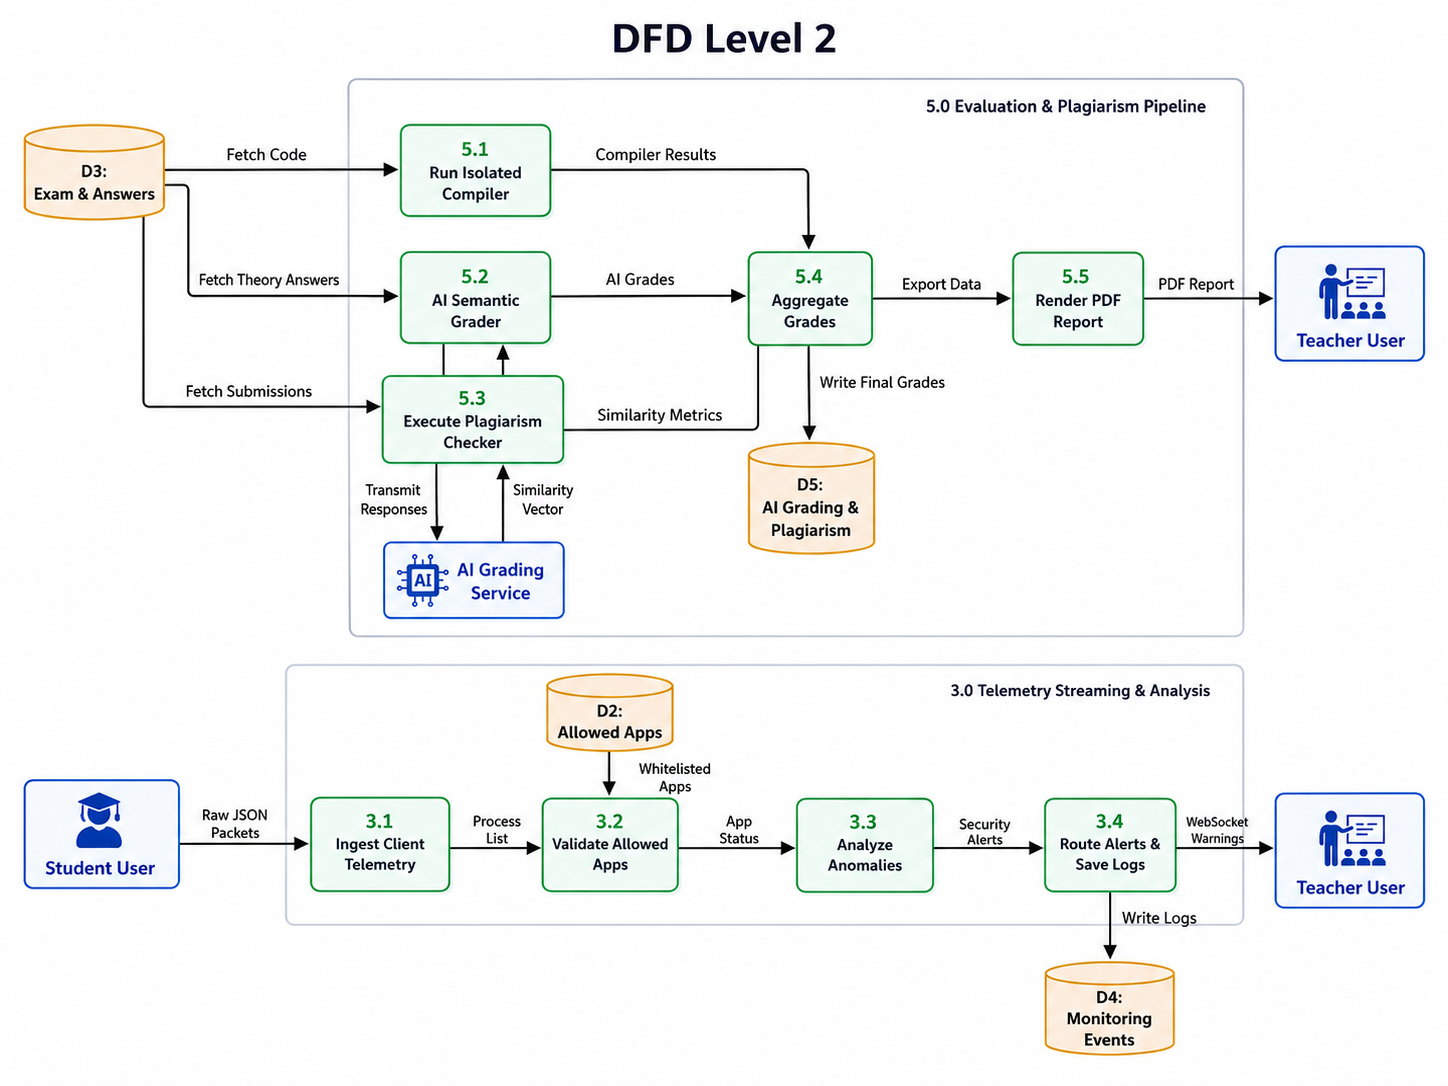
\includegraphics[width=0.97\linewidth]{Figures/dfd_level_2.png}
\caption{Data Flow Diagram (DFD) Level 2 --- Telemetry and Evaluation Processing}
\label{fig:dfd_level_2}
\end{figure}

The detailed flow mapped in Figure~\ref{fig:dfd_level_2} is split into two primary pipelines:

\begin{enumerate}
    \item \textbf{Telemetry Streaming and Analysis (Processes 3.1 to 3.4):}
    \begin{itemize}
        \item \textbf{Process 3.1 (Ingest Client Telemetry):} Receives raw WebSocket JSON packets containing process names, window focus handles, and compressed screenshot payloads from the client.
        \item \textbf{Process 3.2 (Validate Allowed Apps):} Compares the running process names against the exam's whitelisted applications fetched from \texttt{AllowedApps}.
        \item \textbf{Process 3.3 (Analyze Anomalies):} Analyzes camera states and window focus durations. If an unauthorized process is detected or camera frames show missing faces, it generates a security alert.
        \item \textbf{Process 3.4 (Route Alerts and Save Logs):} Writes all telemetry logs to \texttt{MonitoringEvents} and pushes violation alerts to the teacher WebSocket stream.
    \end{itemize}
    \item \textbf{Evaluation and Plagiarism Checking (Processes 5.1 to 5.5):}
    \begin{itemize}
        \item \textbf{Process 5.1 (Run Isolated Compiler):} Launches submitted code files inside isolated Docker containers, compiles the code, executes it against input parameters retrieved from \texttt{TestCases}, and calculates pass rates.
        \item \textbf{Process 5.2 (AI Semantic Grader):} Transmits subjective theory text answers to the semantic similarity engine, which calculates closeness vectors against the teacher's key answers.
        \item \textbf{Process 5.3 (Execute Plagiarism Checker):} Compares submission code ASTs (Abstract Syntax Trees) and text strings pairwise across all class submissions to check for copied content.
        \item \texttt{Process 5.4 (Aggregate Grades):} Consolidates compiling results, AI semantic scores, and plagiarism metrics, writing them to \texttt{AiGradingResults} and \texttt{PlagiarismResults}.
        \item \texttt{Process 5.5 (Render QuestPDF Report):} Fetches consolidated grades, audit overrides, and attendance logs to render a styled PDF report for download.
    \end{itemize}
\end{enumerate}

These Level 2 processes define the core technical operations of the SmartExam system. By mapping data transforms in detail, the modeling ensures that telemetry classification and auto-grading compilation remain robust and scalable under real lab conditions.